\documentclass[10pt]{article}
\usepackage[a4paper,margin=17mm]{geometry}
\usepackage{graphicx,hyperref,booktabs,amsmath}
\hypersetup{colorlinks=true,urlcolor=blue}
\setlength{\parindent}{0pt}\setlength{\parskip}{5pt}
\begin{document}
\begin{center}\Large Branch-local affine consequences\\[3pt]
\normalsize Assignment lifetimes and a fixed-budget regression --- 16 November 2026\end{center}
The Rust bridge specializes original equations at propagation quiescence,
appends conditional affine consequences, and drops their generation before
Undo. A separate BigUint/LIFO checker binds exact premises and invokes the
frozen static coefficient checker. All original variables/equations stay.
Native PCC-20261116-0c76bf; separate native record reader PCC-20261116-10062c.
All standing unsigned/unverified. [pcc:unverified]

\begin{center}\begin{tabular}{lrrr}\toprule
Fixed curve requests, $n=28$ & Root & Unsupported & Cumulative-model cap\\\midrule
Old v1 / exact disabled fork &15&13&0\\
Enabled bridge &13&0&15\\\bottomrule
\end{tabular}\end{center}
All 13 original toy inputs cap, plus two previously completed indexed inputs
(toy00, toy07). The other 11 indexed toy roots and two actual-q1 roots keep
their original node counts. This variant adds no completed-curve node gain
at this fixed budget and loses two baseline roots to caps. Capped shorter
traces are not gains or absence certificates. The 64 MiB ceiling is cumulative
modeled reservations, not measured live memory/RSS. [pcc:unverified]

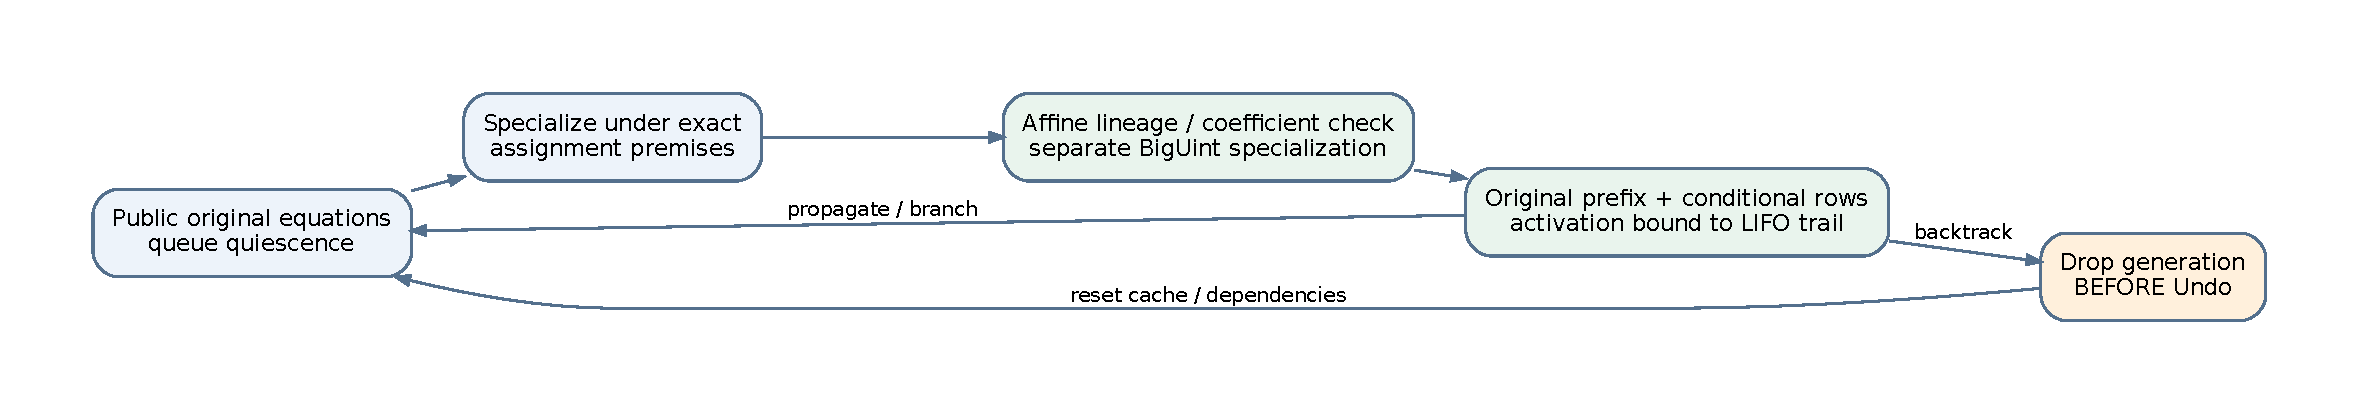
\includegraphics[width=\linewidth,height=39mm,keepaspectratio]{pipeline.pdf}\par
At quiescence before a nonunique branch or Unsupported exit, recompute from
specialized ORIGINAL rows, preserving protected semantic inputs. Conditional
rows are leased to the exact trail. Replacement and rollback discard them and
reset dependency/cache/queue state. This is recomputation, not an incremental
basis. Coefficient/lifetime checking does not prove search completeness or
logical necessity of each decision. [pcc:unverified]

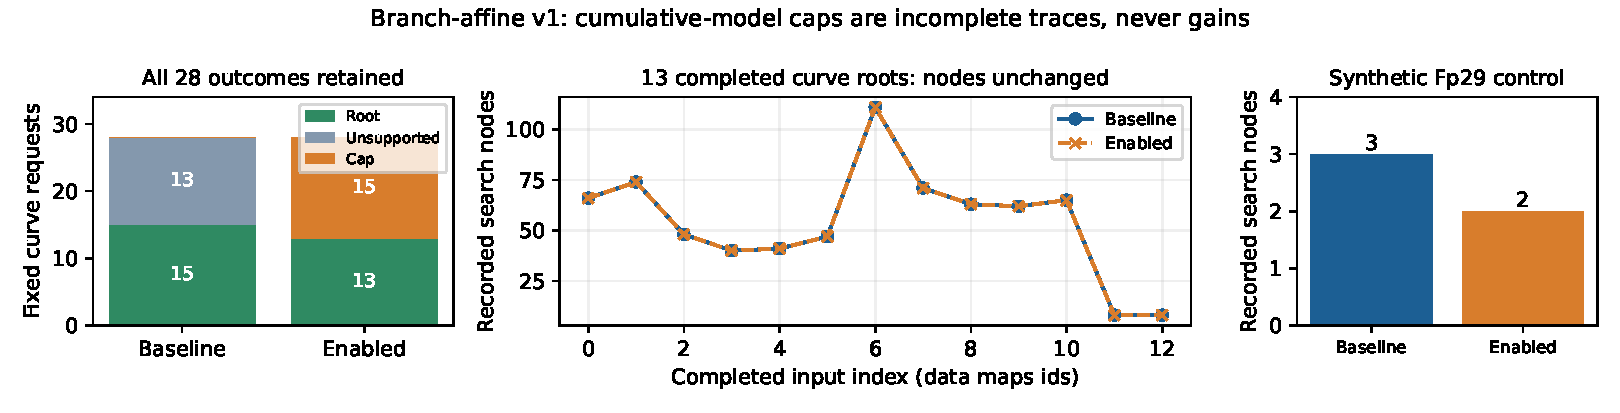
\includegraphics[width=\linewidth]{outcomes.pdf}
Native recorded values only, all 28 curve cases retained; completed-root plot
contains 13 inputs. One synthetic Fp29 conditional-root control changes 3 to 2
nodes and reaches the z0 root before the old solver's z1 root. It is separate
from the curve comparison. No timing, sampling, uncertainty or scaling fit.
[pcc:unverified]

\textbf{Comparator and root checks.} Disabled engine matches unchanged v1
full answers, decisions, counters and schedule on 33 systems. Enabled changes
may change roots/traces. Every returned curve root receives independent
original-equation and native indexed-row/group replay. Solver query arguments
are public System, semantic indices, limits and mode; never a witness, label,
sign, point list or scalar. Index tables are replay-only and unpriced.
[pcc:unverified]

\textbf{Domains.} Toy p101/A95/h(17,12)/a17/q3/k8, arity two, 13 image targets,
distinct raw columns, aliases retained, identity columns excluded. Actual
$p=2^{255}-19$, A486662, $h_{new}=h_{old}^{213156431}$, a60824497/q1/k2, arity two.
This actual domain has TWO columns. Huge original q213156431 six-member
systems receive zero solver calls in this stage. [pcc:unverified]

\newpage
\begin{center}\Large Controls, source identity and next gate\end{center}
\textbf{Bounded controls.} Five Fp29 systems cover coupled/protected linear
equations, conditional root, conditional contradiction then another branch's
root, and underdetermined nonlinear constraints. Original truth enumeration
is 841 assignments per two-variable input and 24,389 per three-variable input.
Each conditional generation is checked over every matching assignment. The
nonlinear case has 28 original roots and remains Unsupported. Eight trace/root
mutations, seven forced caps and four malformed public requests are refused;
omitting Drop before Undo is an explicit corruption. [pcc:unverified]

\textbf{Unchanged budget, incomplete accounting.} Solver limits remain 1024
nodes/depth128/10,000,000 charged diagnostic events/64 MiB cumulative modeled
reservations, 4096 variables/8192 equations/32768 terms/degree2. Extra pass cap
1024 and trace-event cap65536 are finite refusals. Recorded compiler,
specialization/rebuild/trace work is charged. Checker internal arithmetic,
parsing/serialization, actual allocator/container costs, live storage and
original/group replay are not fully priced. These counters are not cold work
or complete field operations. [pcc:unverified]

\textbf{Frozen core.} Composite 98 inputs: unchanged 64-input static context
+34 new (six Rust/Cargo files, 28 exact public requests). All 35 compiled
bindings and five archive round-trips match. No monolithic 98 archive.
Retained 3,432,840-byte executable SHA-256:\\
\texttt{87e5872e4f5743884237b56b740a27be6f03c2e1127adde1ccf60c149ebcfb4f}.\par
Full raw tree 247 files/110,509,160 bytes, one 280,300-byte archive SHA-256:\\
\texttt{5332de1c3b6981ab664cc6e71b1c162996ac7ef812a572a382af5382b27896ad}.\par
Core release library controls/fmt/build/strict all-target Clippy pass locally;
no qualified source/fixture edit afterward. See \path{FROZEN.md},
\path{REPRODUCE.md}, manifests and pre-call data in \path{branch-affine-v1/}.
Artifact storage still requires a genuine exact receipt. [pcc:unverified]

\textbf{Separate native post-call reader.} One Python status-grouping
diagnostic is excluded from acceptance. The separately frozen Rust reader
hashes all 247 raw members, compares all 33 old/disabled artifacts and computes
these totals. Its one source/binary/39rlib bindings and pre-call are separate
from the core 98 inputs. First reader build failed on an assumed release/deps
directory; actual Cargo build/out paths fixed the lookup without source changes.
All logs and the complete 11,020-byte audit round remain. No solver rerun for
aggregation. This reader verifies records, not execution or solver/counter
correctness. See \path{POSTCALL_PROVENANCE.md}. [pcc:unverified]

\textbf{Prior art.} Soos, Nohl, Castelluccia, \emph{Extending SAT Solvers to
Cryptographic Problems}, section3.2 pp248--249:
\url{https://www.msoos.org/wordpress/wp-content/uploads/2011/03/Extending_SAT_2009.pdf}.
Their GF2 integration invokes Gaussian reasoning at quiescence and restores
matrices on backtracking; fewer branches need not reduce time. Shoup NTBv2
section14.4 pp388--391 covers classical row operations:
\url{https://shoup.net/ntb/ntb-v2.pdf}.
KB MCP/wrapper unavailable; first guessed paper URL404 was corrected via the
author's index, and the primary section was read. No novelty for this hybrid.

\textbf{Next discriminating gate.} This closes the fixed-control pruning claim
for this recompute-every-quiescence implementation and budget. It does not
disprove branch-local reasoning or an index-calculus family. Share the immutable
prefix and update/undo a bounded sparse component; account for row/certificate/
checker and allocation work before comparison. A cutoff requires a new frozen
schedule, not reuse of a cipher-specific optimum. No successor campaign is
scheduled by the CI checker. Canonical cost/exponent charts and benchmarks stay
unchanged: no admitted performance datum. Original criteria and source pins
remain unchanged. [pcc:unverified]
\end{document}
